
	\documentclass{article}
	\usepackage{amsmath,amssymb}
	\usepackage{enumitem}
	\usepackage{blindtext}
	\usepackage{booktabs}
	\usepackage{graphicx}
	\usepackage{xcolor}
	\usepackage[vmargin = 1.5in, top = 1in, bottom = 1.2in, letterpaper]{geometry}
	\usepackage{listings}
	\usepackage{courier}

	\lstset{
	basicstyle = \small\tt,
	keywordstyle = \tt\color{blue},
	commentstyle = \tt\color[cmyk]{1,0,1,0},
	stringstyle = \tt\color[RGB]{128,0,0},
	%frame = single,
	backgroundcolor = \color[RGB]{245,245,244},
	breaklines,
	extendedchars = false,
	xleftmargin = 2em,
	xrightmargin = 2em,
	aboveskip = 1em,
	tabsize = 4,
	showspaces = false
	}
	\begin{document}
	
	% \newfontfamily\courier{Courier New}

	
	\title{STAT 579 Homework 2}
	\author{Yifan Zhu}
	\maketitle
	
	\begin{enumerate}[leftmargin = 0 em, label = \arabic*., font = \bfseries]

	\item \begin{enumerate}
	\item 
	\begin{lstlisting}[language = R]
> year <- seq(from = 2008, to = 1948, by = -4) # year column
> winner <- c(185, 182, 182, 189, 189, 188, 185, 185, 177, 182, 182, 193, 183, 179, 179, 175) # winners' heights
> opponent <- c(175, 193, 185, 187, 188, 173, 180, 177, 183, 185, 180, 180, 182, 178, 178, 173) # opponents' heights
> height <- data.frame(year = year, winner = winner, opponent = opponent)
> height
   year winner opponent
1  2008    185      175
2  2004    182      193
3  2000    182      185
4  1996    189      187
5  1992    189      188
6  1988    188      173
7  1984    185      180
8  1980    185      177
9  1976    177      183
10 1972    182      185
11 1968    182      180
12 1964    193      180
13 1960    183      182
14 1956    179      178
15 1952    179      178
16 1948    175      173
	\end{lstlisting}

	\item 
\begin{lstlisting}[language = R]
> difference <- winner - opponent # calculate the difference of heights
> height1 <- data.frame(year = year, winner = winner, opponent = opponent, difference = difference) # create new date frame with difference of heights
> height1
   year winner opponent difference
1  2008    185      175         10
2  2004    182      193        -11
3  2000    182      185         -3
4  1996    189      187          2
5  1992    189      188          1
6  1988    188      173         15
7  1984    185      180          5
8  1980    185      177          8
9  1976    177      183         -6
10 1972    182      185         -3
11 1968    182      180          2
12 1964    193      180         13
13 1960    183      182          1
14 1956    179      178          1
15 1952    179      178          1
16 1948    175      173          2
\end{lstlisting}

\item
\begin{lstlisting}[language = R]
> taller.won = (difference > 0) # difference > 0 means the winner being taller is TRUE.
> height <- data.frame(height, taller.won = taller.won) # add the colume to the data frame in (a)
> height
   year winner opponent taller.won
1  2008    185      175       TRUE
2  2004    182      193      FALSE
3  2000    182      185      FALSE
4  1996    189      187       TRUE
5  1992    189      188       TRUE
6  1988    188      173       TRUE
7  1984    185      180       TRUE
8  1980    185      177       TRUE
9  1976    177      183      FALSE
10 1972    182      185      FALSE
11 1968    182      180       TRUE
12 1964    193      180       TRUE
13 1960    183      182       TRUE
14 1956    179      178       TRUE
15 1952    179      178       TRUE
16 1948    175      173       TRUE
\end{lstlisting}

\item
\begin{lstlisting}[language = R]
> count <- table(height$taller.won) # table function for counts
> percentage <- count / length(height$taller.won) # calculate the percentage
> percentage

FALSE  TRUE 
 0.25  0.75 
\end{lstlisting}
Most winners (75\%) are taller than their opponents.

\item
\begin{lstlisting}[language = R]
> barplot(height = rev(height1$difference), names.arg = rev(height$year)) # reverse and plot
\end{lstlisting}
\begin{center}
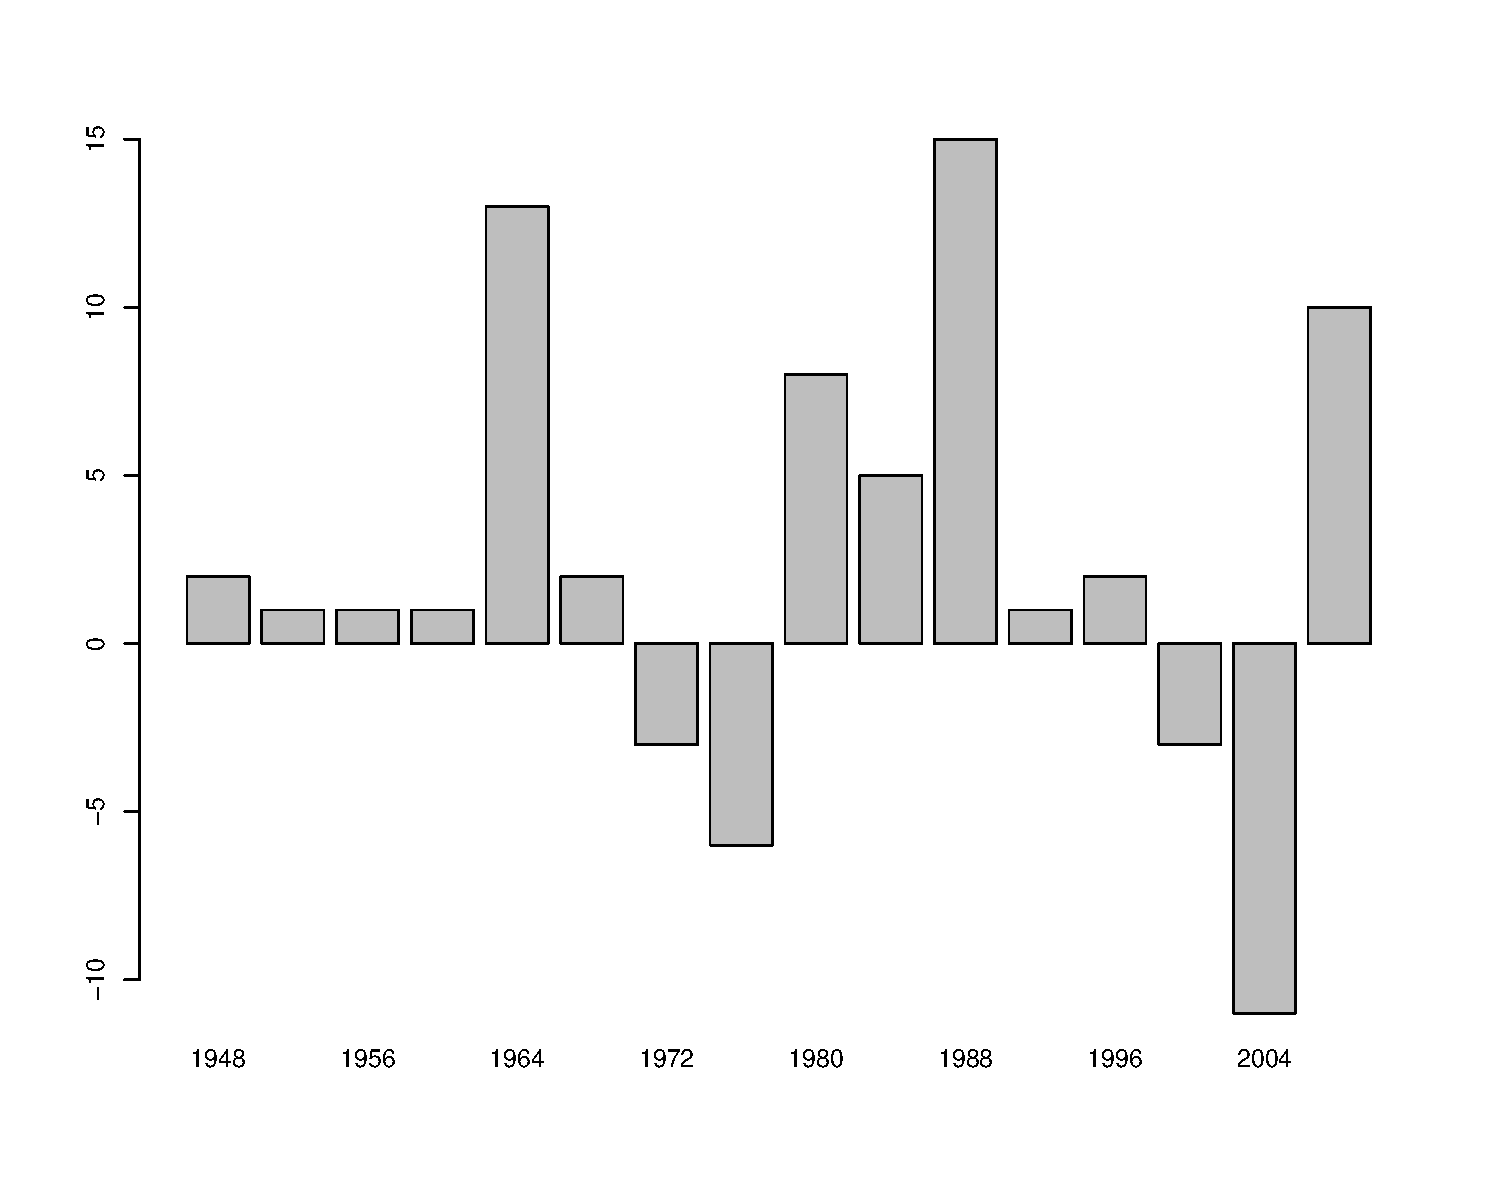
\includegraphics[width = 0.52\textwidth]{1(e)barplot.eps}
\end{center}

 	\end{enumerate}
\item \begin{enumerate} 
\item
\begin{lstlisting}[language = R]
> student <- read.table(file = "C:/Users/fanne/Desktop/STAT579/students.txt", header = T) # read data 

> MeanHeight <- mean(student$height) #calculate the mean height
> MeanHeight
[1] 169.7647
> MeanShoesSize <- mean(student$shoesize) #calculate the mean shoesize
> MeanShoesSize
[1] 40.47059
> SDHeight <- sd(student$height) # standard deviation of height
> SDHeight
[1] 7.578996
> SDShoesSize <- sd(student$shoesize) # standard deviation of shoesize
> SDShoesSize
[1] 2.695312
\end{lstlisting}

\item
\begin{lstlisting}[language = R]
> table(student$gender) #count the number of male and female students

female   male 
     9      8 
\end{lstlisting}
9 female students and 8 male students.

\item
\begin{lstlisting}[language = R]
> populationColor <- ifelse(student$population == "kuopio", c("blue"), c("red")) # recode the population variable
> students_new <- student # create new dataset "students_new"
> students_new$population <- populationColor # use the recoded population cariable for the new dataset
> students_new
   height shoesize gender population
1     181       44   male       blue
2     160       38 female       blue
3     174       42 female       blue
4     170       43   male       blue
5     172       43   male       blue
6     165       39 female       blue
7     161       38 female       blue
8     167       38 female        red
9     164       39 female        red
10    166       38 female        red
11    162       37 female        red
12    158       36 female        red
13    175       42   male        red
14    181       44   male        red
15    180       43   male        red
16    177       43   male        red
17    173       41   male        red
\end{lstlisting}

\item
\begin{lstlisting}[language = R]
> female <- subset(student, gender == "female") # female subset
> female
   height shoesize gender population
2     160       38 female     kuopio
3     174       42 female     kuopio
6     165       39 female     kuopio
7     161       38 female     kuopio
8     167       38 female    tampere
9     164       39 female    tampere
10    166       38 female    tampere
11    162       37 female    tampere
12    158       36 female    tampere
> write.table(female, "C:/Users/fanne/Desktop/STAT579/female.txt", quote = F, row.names = F) # export to female.txt
> 
> male <- subset(student, gender == "male") #male subset
> male
   height shoesize gender population
1     181       44   male     kuopio
4     170       43   male     kuopio
5     172       43   male     kuopio
13    175       42   male    tampere
14    181       44   male    tampere
15    180       43   male    tampere
16    177       43   male    tampere
17    173       41   male    tampere
> write.table(male, "C:/Users/fanne/Desktop/STAT579/male.txt", quote = F, row.names = F) # export to male.txt
\end{lstlisting}

\item
\begin{lstlisting}[language = R]
> MedianHeight <- median(student$height) #calculate the median height
> below <- subset(student, height < MedianHeight)
> below
   height shoesize gender population
2     160       38 female     kuopio
6     165       39 female     kuopio
7     161       38 female     kuopio
8     167       38 female    tampere
9     164       39 female    tampere
10    166       38 female    tampere
11    162       37 female    tampere
12    158       36 female    tampere
> write.csv(below, "C:/Users/fanne/Desktop/STAT579/below.csv", quote = F, row.names = F) # export to below.csv
> 
> abovem <- subset(student, height > MedianHeight)
> abovem
   height shoesize gender population
1     181       44   male     kuopio
3     174       42 female     kuopio
5     172       43   male     kuopio
13    175       42   male    tampere
14    181       44   male    tampere
15    180       43   male    tampere
16    177       43   male    tampere
17    173       41   male    tampere
> write.csv(abovem, "C:/Users/fanne/Desktop/STAT579/abovem.csv", quote = F, row.names = F) # export to abovem.csv
\end{lstlisting}

\end{enumerate}

\item \begin{enumerate}
	\item 
\begin{lstlisting}[language = R]
> cars <- read.table(file = "http://maitra.public.iastate.edu/stat579/datasets/cars.dat", header = T) # read the file
\end{lstlisting}

\item
\begin{lstlisting}[language = R]
> attach(cars) #attach the dataframe
\end{lstlisting}

\item
\begin{lstlisting}[language = R]
> speed_ft_per_s <- 5280 * speed / 3600 # convert speed to feet per second
> speed_ft_per_s
 [1]  5.866667  5.866667 10.266667 10.266667 11.733333 13.200000 14.666667 14.666667 14.666667 16.133333 16.133333 17.600000 17.600000
[14] 17.600000 17.600000 19.066667 19.066667 19.066667 19.066667 20.533333 20.533333 20.533333 20.533333 22.000000 22.000000 22.000000
[27] 23.466667 23.466667 24.933333 24.933333 24.933333 26.400000 26.400000 26.400000 26.400000 27.866667 27.866667 27.866667 29.333333
[40] 29.333333 29.333333 29.333333 29.333333 32.266667 33.733333 35.200000 35.200000 35.200000 35.200000 36.666667
\end{lstlisting}

\item
\begin{lstlisting}[language = R]
> plot(x = dist, y = speed_ft_per_s, xlab = "Distance (feet)", ylab = "Speed (feet/second)", main = "Speed (feet/second) vs. Distance (feet)") # plot speed (feet/second) against distance (feet)
\end{lstlisting}

\begin{center}
	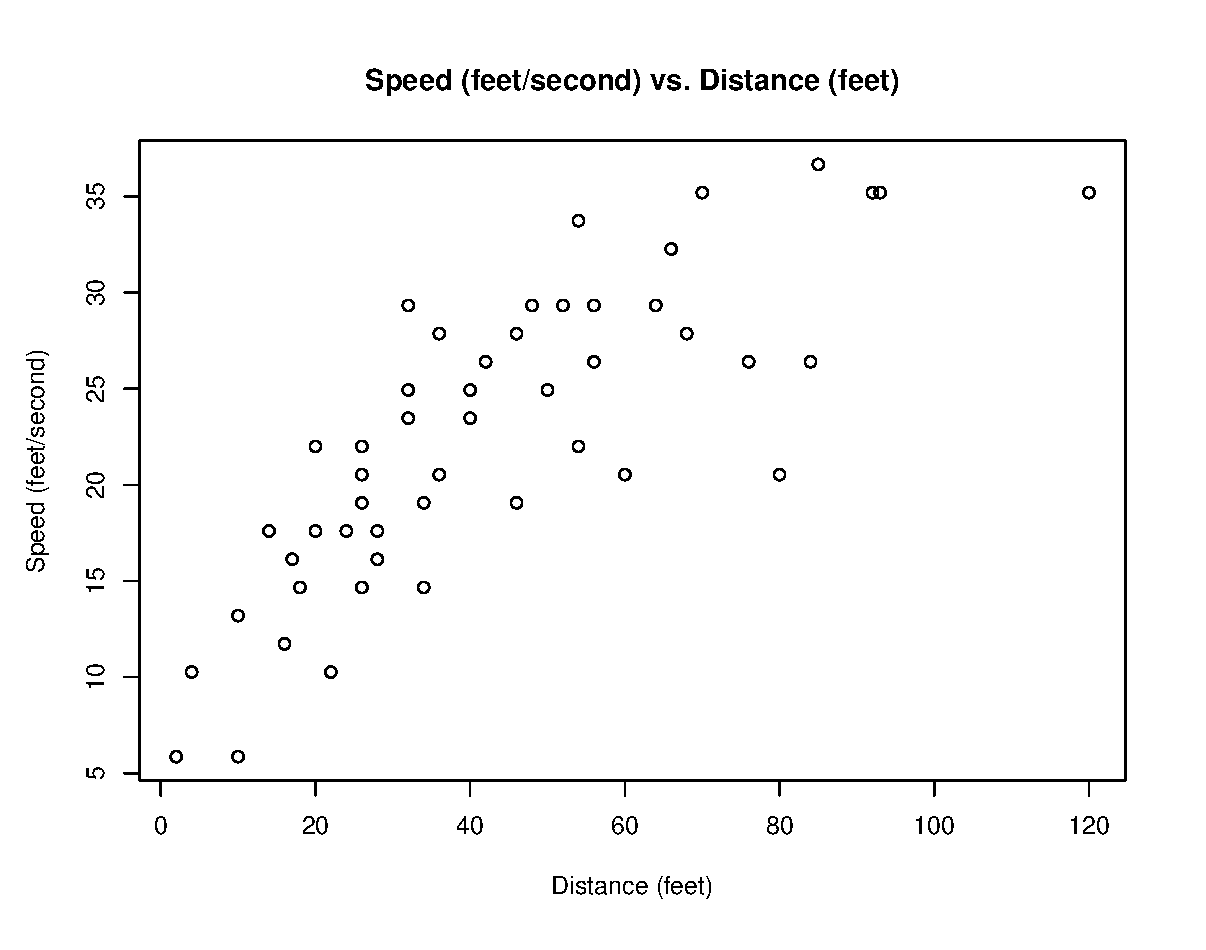
\includegraphics[width = 0.8\textwidth]{speed_vs_dist_ft.eps}
\end{center}

\item
\begin{lstlisting}[language = R]
> speed_m_per_s <- speed * 1.6093 * 1000 / 3600 # convert speed to meter per second
> speed_m_per_s
 [1]  1.788111  1.788111  3.129194  3.129194  3.576222  4.023250  4.470278  4.470278  4.470278  4.917306  4.917306  5.364333  5.364333
[14]  5.364333  5.364333  5.811361  5.811361  5.811361  5.811361  6.258389  6.258389  6.258389  6.258389  6.705417  6.705417  6.705417
[27]  7.152444  7.152444  7.599472  7.599472  7.599472  8.046500  8.046500  8.046500  8.046500  8.493528  8.493528  8.493528  8.940556
[40]  8.940556  8.940556  8.940556  8.940556  9.834611 10.281639 10.728667 10.728667 10.728667 10.728667 11.175694
> 
> dist_m <- dist / 5280 * 1.6093 * 1000  # convert distance to meter
> dist_m
 [1]  0.6095833  3.0479167  1.2191667  6.7054167  4.8766667  3.0479167  5.4862500  7.9245833 10.3629167  5.1814583  8.5341667  4.2670833
[13]  6.0958333  7.3150000  8.5341667  7.9245833 10.3629167 10.3629167 14.0204167  7.9245833 10.9725000 18.2875000 24.3833333  6.0958333
[25]  7.9245833 16.4587500  9.7533333 12.1916667  9.7533333 12.1916667 15.2395833 12.8012500 17.0683333 23.1641667 25.6025000 10.9725000
[37] 14.0204167 20.7258333  9.7533333 14.6300000 15.8491667 17.0683333 19.5066667 20.1162500 16.4587500 21.3354167 28.0408333 28.3456250
[49] 36.5750000 25.9072917
\end{lstlisting}

\item
\begin{lstlisting}[language = R]
> detach()
\end{lstlisting}

\item
\begin{lstlisting}[language = R]
> plot(x = dist_m, y = speed_m_per_s, xlab = "Distance (meter)", ylab = "Speed (meter/second)", main = "Speed (meter/second) vs. Distance (meter)") # plot speed (meter/second) against distance (meter)
\end{lstlisting}

\begin{center}
	\includegraphics[width = 0.8\textwidth]{speed-vs-distance-m.eps}
\end{center}

\item
\begin{lstlisting}[language = R]
> pdf(file = "C:/Users/fanne/Desktop/STAT579/speed-vs-distance.pdf", onefile = T) # print to one file
> plot(x = cars$dist, y = speed_ft_per_s, xlab = "Distance (feet)", ylab = "Speed (feet/second)", main = "Speed (feet/second) vs. Distance (feet)") # plot speed (feet/second) against distance (feet)
> plot(x = dist_m, y = speed_m_per_s, xlab = "Distance (meter)", ylab = "Speed (meter/second)", main = "Speed (meter/second) vs. Distance (meter)") # plot speed (meter/second) against distance (meter)
> dev.off()
\end{lstlisting}

Except for the measurement, they look the same.
\end{enumerate}

\item
\begin{lstlisting}[language = R]
> activation <- matrix(scan("C:/Users/fanne/Desktop/STAT579/activ.dat"), nrow = 83, ncol = 108, byrow = T) # read activation data
Read 8964 items
> anatomic <- matrix(scan("C:/Users/fanne/Desktop/STAT579/anat.dat"), nrow = 83, ncol = 108, byrow = T) # read anatomic data
Read 8964 items
> image(-activation, axes = F, col = gray.colors(n = 255, start = 0.1, end = 1)) # plot the image of activation
> contour(anatomic, axes = F, drawlabels = F, add = T) # overlay contour of anatomic atop activation image
\end{lstlisting}

\begin{center}
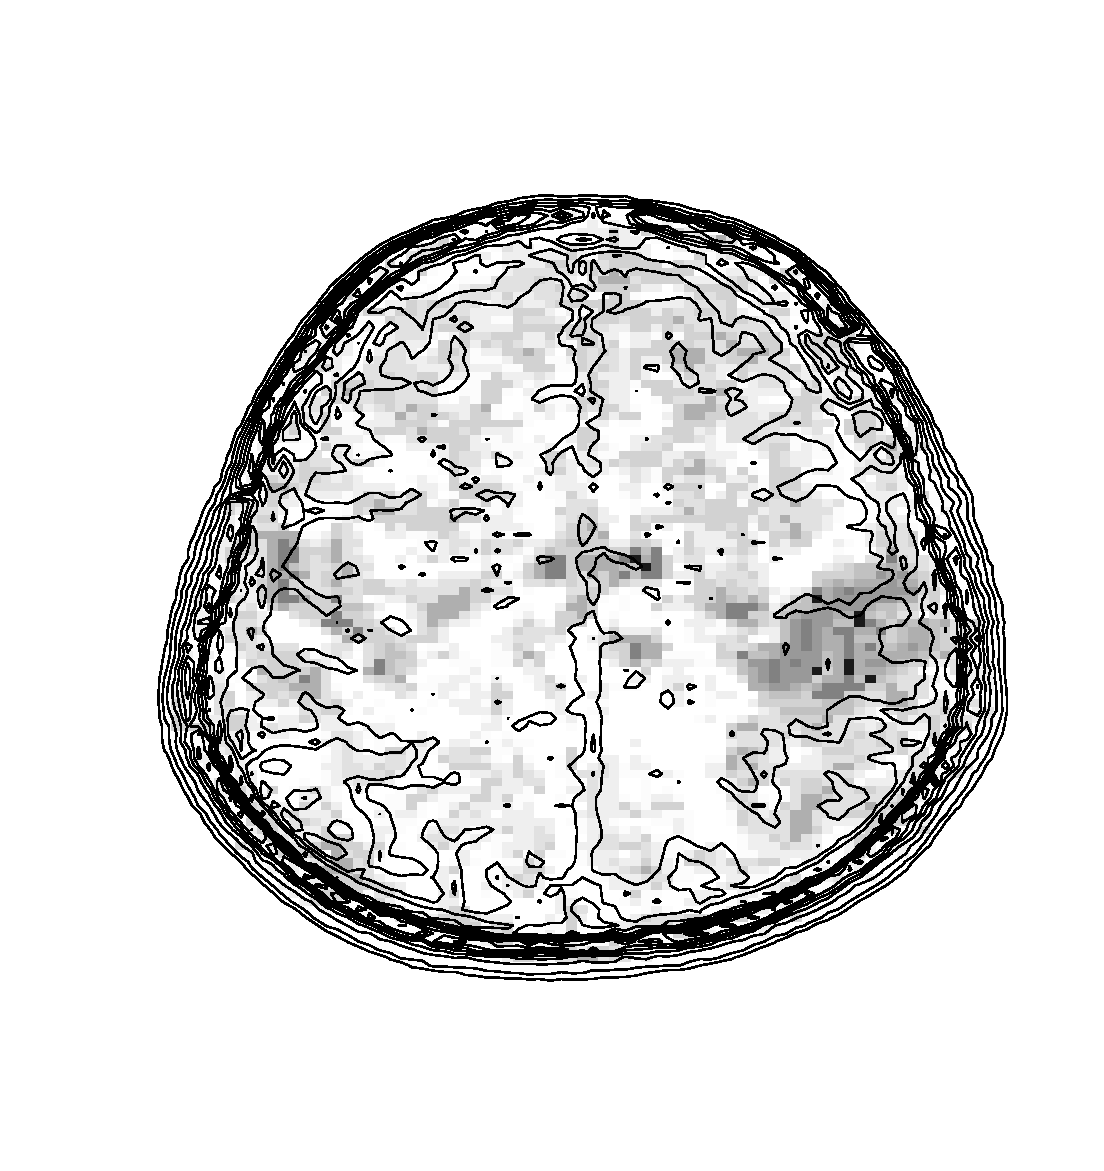
\includegraphics[width = 0.6\textwidth]{brain.eps}
\end{center}
\end{enumerate}
	
	
	\end{document}